\documentclass[10pt,a4paper,parskip=full*,DIV=11]{scrartcl}
\usepackage[utf8]{inputenc}
\usepackage[T1]{fontenc}
\usepackage[french]{babel}
\frenchsetup{StandardItemLabels=true}
\usepackage{textcomp}
\usepackage{lmodern}
\usepackage{graphicx}
\usepackage[dvipsnames,svgnames]{xcolor}
\usepackage{microtype}
\usepackage{hyperref} \hypersetup{colorlinks=true,linkcolor=Brown,urlcolor=Navy,
breaklinks=true,pdfstartview=XYZ}
\usepackage{enumitem}
\usepackage{listings}
\lstset{
upquote = true,
columns = flexible,
basicstyle = \ttfamily,
keepspaces=true,
language = sql,
backgroundcolor = \color{Navy!10},
keywordstyle = \color{ForestGreen}\bfseries,
numbers=left, numberstyle=\tiny,
tabsize = 4,
}

\title{Rapport BD Librairie}
\author{Jeanne BARASTIER, Yann ROBLIN, Tom BARTIER}
\begin{document}
\maketitle
\begin{abstract}
    Dans le cadre du cours de remise à niveau de la première année de master nous devons réaliser une base de données en groupe. Le but est d’introduire, et de familiariser 
    les personnes ne venant pas de la licence informatique aux bases de la conception d’une base de données, 
    aux commandes et langage SQL et à la création d’une application simple via le langage de programmation python. 
    Le projet se sépare en deux étapes distinctes. La première étape consiste à concevoir et construire une base de 
    données de notre choix. La deuxième étape consiste à réaliser une application qui exploitera cette base de données.
\end{abstract}

\newpage
\tableofcontents
\newpage

\section{Consignes}
Le travail qui nous est demandé n’est pas uniquement la création d’une base de 
données mais bel et bien la réalisation d’un petit projet. C’est pour cela qu’en 
plus d’une série de tables nous devons réaliser une série de tâches. Tout d’abord nous 
devons choisir un contexte pour notre base de données. Après en avoir choisi un, il faut
 créer un cahier des charges afin de définir nos objectifs. Ensuite vient la conception
  du Modèle Entité Association (MEA) de notre base de données. Une fois les étapes 
  précédentes réalisées nous pouvons passer à la partie SQL du projet. Tout d’abord il 
  y a la création des tables décrites dans le MEA. Une fois créées, nous devons remplir
   les tables à l’aide de requêtes. En plus des tables nous devons ajouter au moins deux
    déclencheurs. Une fois la base créée nous écrirons une série pertinente 
    d’instructions afin de la valider ainsi que deux exemples de cas d’utilisations 
    concurrentes qui poseraient problème. Tout ceci est à terminer pour fin septembre. 
Une application exploitant la base de données doit être présentée fin octobre.

\section{Librairie}
Le projet qu’on a choisi est la création d’une application à destination du personnel d’une librairie non initié au SQL. Elle doit principalement permettre de mettre à jour 
et consulter les stocks, les achats et les emprunts de livres. Nous avons fait ce choix car il s’agit d’un exemple simple et 
longuement traité pendant la licence. Comme il s’agit d’un projet d’initiation, la base de données sera assez simple et ne comportera donc que les éléments que nous jugeons essentiels.

\section{Cahier des charges}

\begin{itemize}
    \item L’application sera destinée au personnel d’une librairie non initié à SQL.
    \item Il faut que l'application soit ergonomique, simple d'utilisation tout en restant fonctionnelle.
    \item Elle permet de consulter les différentes tables de la base de données via des actions simples par un non initié à SQL.
    \item Elle doit permettre au personnel de modifier les différentes tables de la base de données via des actions simples pour un non initié à SQL.
    \item Chaque action réalisée sur l'application notamment concernant la modification des tables doit avoir un retour visuel.
\end{itemize}

% \newpage

\section{La base de données}

\begin{itemize}[itemsep = 1em]
    \item Une table « Auteurs » qui contient les informations de chaque auteur des livres proposés à la vente ou à l’emprunt. Chaque auteur est différencié par un identifiant unique de 
    type entier. Un auteur possède un nom, un prénom, une date de naissance, la date de sa mort qui est vide si l’auteur est en vie, et une nationalité.\
    \
    \item Une table « Editeurs » qui contient une liste d’éditeurs. Chaque éditeur est différencié par un identifiant unique. Un éditeur possède un nom, le nom et prénom du patron, et le nom du 
    pays dans lequel est installé la direction.\
    \
    \item Une table « Livres » qui contient les références des livres de la librairie proposés à la vente ou à l’emprunt. L’ISBN sera l’identifiant unique pour chaque référence de livre. 
    Un livre possède un titre, l’identifiant unique de la table Auteurs de l’auteur qui l’a écrit, 
    l’identifiant unique de la table Editeur de l’éditeur qui le publie, une date de sortie, le genre, la quantité disponible dans les rayons de la librairie et un prix d’achat.\
    \
    \item Une table « Clients » qui contient les informations des clients. Chaque client est différencié par un identifiant unique de type entier. Un client possède un nom, un prénom et une date de 
    naissance.\
    \
    \item Une table « Achat » qui contient l’historique d’achat de la librairie. Un achat est différencié par un numéro unique. Pour chaque achat il est renseigné l’identifiant unique du client, l’ISBN du livre, la date d’achat, 
    la quantité d’exemplaires achetés et le prix total.\
    \
    \item Une table « Emprunt » qui contient l’historique d’emprunts. Chaque emprunt est différencié par un numéro unique. Pour chaque emprunt il est renseigné l’ISBN du livre, la date de début 
    de l’emprunt, la date de fin de l’emprunt, le statut de l’emprunt c’est-à-dire si le livre est rendu ou non, et l’état du livre. L’état du livre et le statut de l’emprunt sont déclarés avec
     deux nouveaux domaines. L’état du livre pourra être bon, ou mauvais au début de l’emprunt et sera mis à jour à la fin. Si le livre
      est rendu en retard, la date de fin de l’emprunt sera décalée au jour du rendu. Si le livre est rendu en avance, la date de fin sera aussi modifiée au jour 
      où le livre a été rendu.
    
\end{itemize}

\begin{figure}
    \centering
    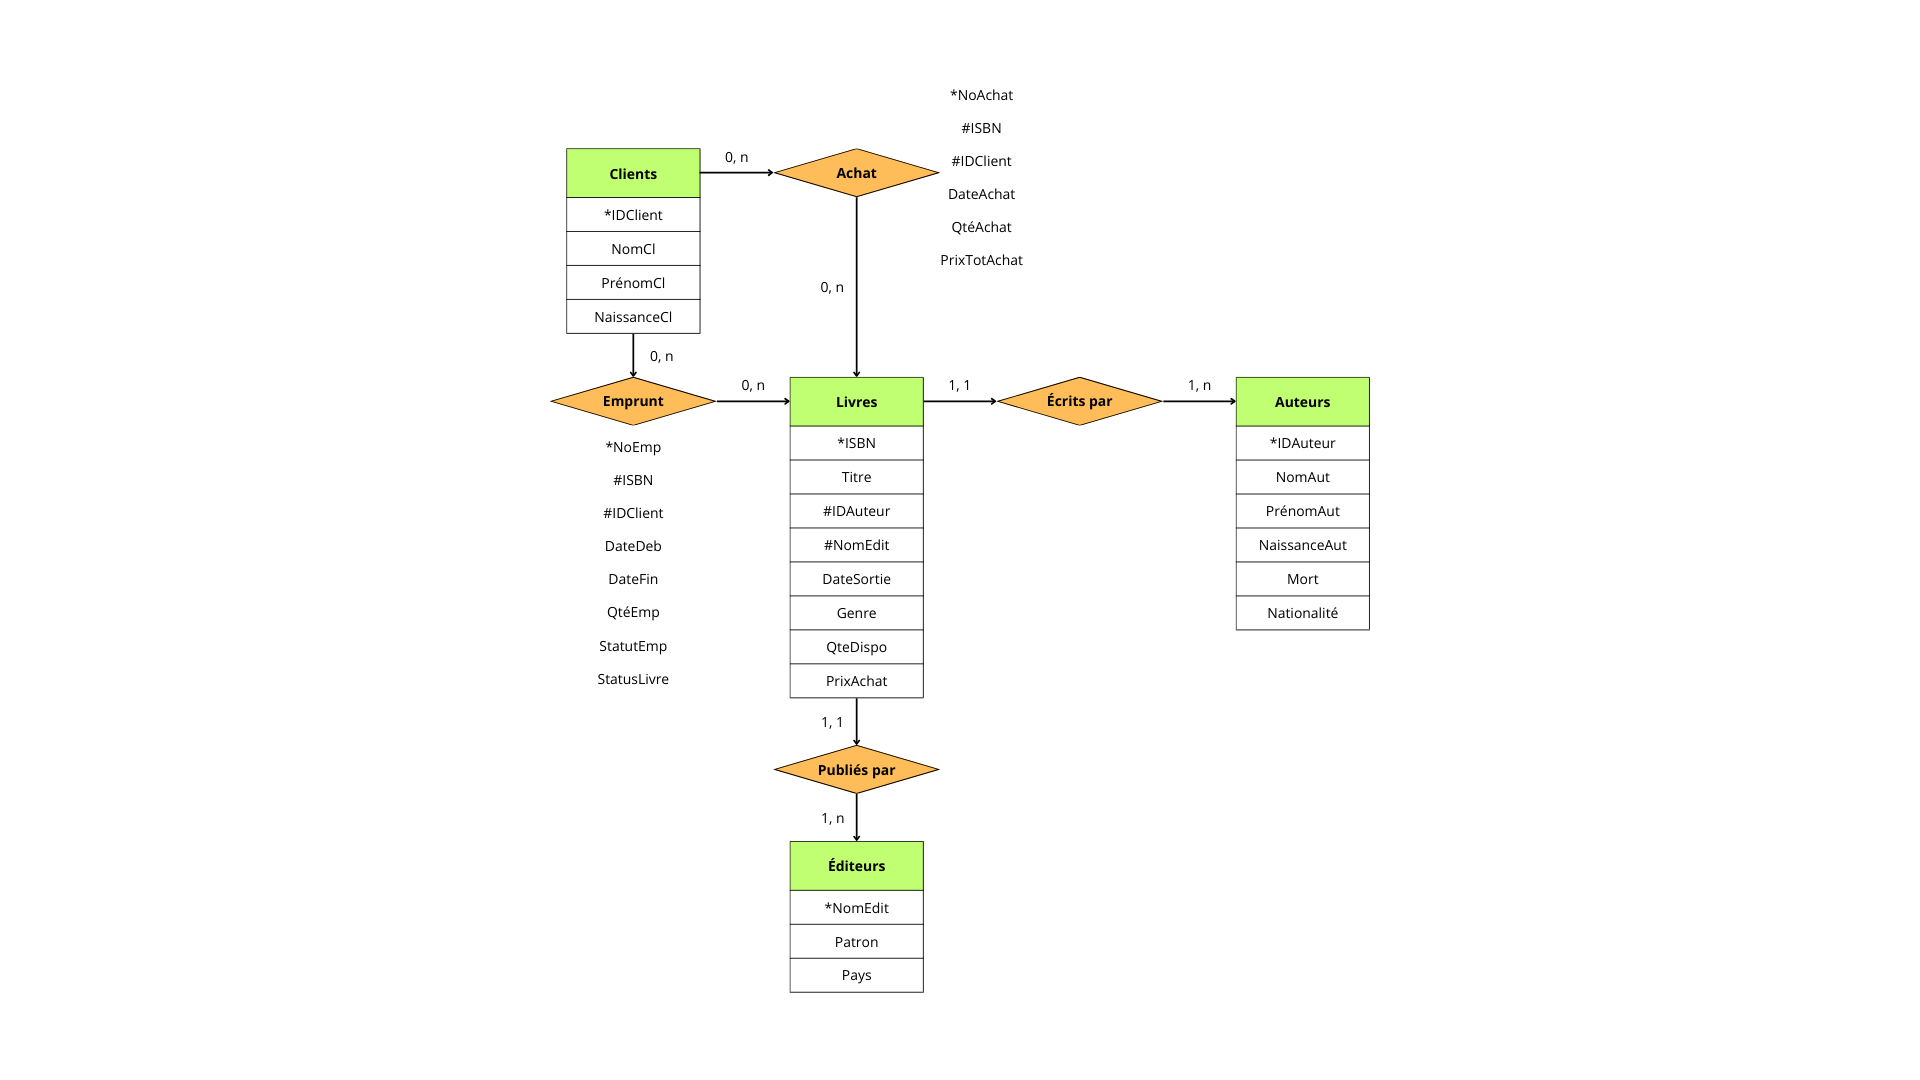
\includegraphics[trim=6cm 0cm 5cm 0cm, clip, width=1.2\textwidth]{MEA_BD}
    \caption{Modèle Entité Association}\label{fig.mea}
\end{figure}

\begin{lstlisting}
CREATE DOMAIN typeEtat
AS VARCHAR(20) 
CHECK(VALUE IN('bon','degrade','perdu'));

CREATE DOMAIN typeEmp
AS VARCHAR(20) 
CHECK(VALUE IN('rendu','non rendu'));
\end{lstlisting}

\section{Déclencheurs}
Nous avons créé plusieurs déclencheurs qui mettent à jour les tables ou les complètent en fonction de certaines actions.

	Le premier déclencheur s’enclenche à chaque insertion dans la table achat. Il permet de vérifier qu’il y ait assez de stock pour la commande, puis dans un second temps de calculer le 
    prix total d’un achat grâce à la quantité d’exemplaires et le prix unitaire d’un livre. Si les stocks tombent à zéro, ils sont automatiquement réapprovisionnés avec cinq nouveaux 
    exemplaires. Comme il s’agit d’une simulation simplifiée nous considérons qu’une commande à un fournisseur est automatiquement faite et qu’elle est instantanément livrée.

Le deuxième déclencheur se déclenche lors d’un nouvel emprunt. Il vérifie qu’il y ait assez de stock, et met à jour la quantité d’exemplaires.

Le troisième déclencheur s’enclenche après qu’un emprunt soit rendu. Il met à jour le statut à "rendu" et met à jour la quantité en stock.

\section{Requêtes}
Afin de prouver la pertinence et les possibilités de notre base de données, nous avons écrit un certain nombre de requêtes. Voir fichier joint.

\section{Concurrence}
Première situation :

Nous avons 2 vendeurs, le premier vendeur reçoit un coup de téléphone d'un client qui demande un livre, le vendeur consulte la table Livres (Lecture) et voit qu'il en reste un exemplaire, le client
 demande qu'on lui mette de côté le livre.
Au même moment un client entre dans le magasin et achète le livre, le vendeur met à jour la table Livres (écriture), le livre est en rupture, le premier vendeur veut mettre à jour la table Livres 
pour l'achat du client qui l'a appelé mais il rencontre une erreur car le
livre est passé en rupture.

Deuxième situation :

Un vendeur vient de recevoir une livraison, il veut donc modifier la quantité disponible d'un livre (écriture). Au même moment, un client veut acheter ce livre (et donc modifier la quantité aussi, 
en écriture). Le SGBD va donc traiter les requêtes en série, d'abord la première puis la seconde.

\section{Pour aller plus loin}
Suite à nos rélfexions après avoir mis en place la BDD, nous nous sommes rendus compte des imperfections de celle-ci, nous aurions pu par exemple :
permettre à un livre d'être écrit par plusieurs auteurs, mettre plusieurs livres sur un même numéro d'achat, différencier chaque exemplaire d'un même livre pour préciser son état lors d'un emprunt,
mettre en place un système de pénalité pour les livres rendus en retard.

\section{Conclusion}
Maintenant que nous partons sur de bonnes bases, il nous reste à mettre en place un exemple concret d'une telle application. Dans notre cas nous allons partir sur une application Python Tkinter qui sera
connectée à la base de données (qui tournera en local sur la même machine).
\end{document}
